\documentclass{sigchi}

% Use this section to set the ACM copyright statement (e.g. for
% preprints).  Consult the conference website for the camera-ready
% copyright statement.

% Copyright
\CopyrightYear{2021}
%\setcopyright{acmcopyright}
\setcopyright{acmlicensed}
%\setcopyright{rightsretained}
%\setcopyright{usgov}
%\setcopyright{usgovmixed}
%\setcopyright{cagov}
%\setcopyright{cagovmixed}
% DOI
\doi{https://doi.org/10.1145/3313831.XXXXXXX}
% ISBN
\isbn{978-1-4503-6708-0/20/04}
%Conference
\conferenceinfo{CHI'21,}{May 8--13, 2021, Yokohama, Japan (Virtual)}
%Price
\acmPrice{\$15.00}

% Use this command to override the default ACM copyright statement
% (e.g. for preprints).  Consult the conference website for the
% camera-ready copyright statement.

%% HOW TO OVERRIDE THE DEFAULT COPYRIGHT STRIP --
%% Please note you need to make sure the copy for your specific
%% license is used here!
% \toappear{
% Permission to make digital or hard copies of all or part of this work
% for personal or classroom use is granted without fee provided that
% copies are not made or distributed for profit or commercial advantage
% and that copies bear this notice and the full citation on the first
% page. Copyrights for components of this work owned by others than ACM
% must be honored. Abstracting with credit is permitted. To copy
% otherwise, or republish, to post on servers or to redistribute to
% lists, requires prior specific permission and/or a fee. Request
% permissions from \href{mailto:Permissions@acm.org}{Permissions@acm.org}. \\
% \emph{CHI '16},  May 07--12, 2016, San Jose, CA, USA \\
% ACM xxx-x-xxxx-xxxx-x/xx/xx\ldots \$15.00 \\
% DOI: \url{http://dx.doi.org/xx.xxxx/xxxxxxx.xxxxxxx}
% }

% Arabic page numbers for submission.  Remove this line to eliminate
% page numbers for the camera ready copy
% \pagenumbering{arabic}

% Load basic packages
\usepackage{balance}       % to better equalize the last page
\usepackage{graphics}      % for EPS, load graphicx instead 
\usepackage[T1]{fontenc}   % for umlauts and other diaeresis
\usepackage{txfonts}
\usepackage{mathptmx}
\usepackage[pdflang={en-US},pdftex]{hyperref}
\usepackage{color}
\usepackage{booktabs}
\usepackage{textcomp}

% Some optional stuff you might like/need.
\usepackage{microtype}        % Improved Tracking and Kerning
% \usepackage[all]{hypcap}    % Fixes bug in hyperref caption linking
\usepackage{ccicons}          % Cite your images correctly!
% \usepackage[utf8]{inputenc} % for a UTF8 editor only

% If you want to use todo notes, marginpars etc. during creation of
% your draft document, you have to enable the "chi_draft" option for
% the document class. To do this, change the very first line to:
% "\documentclass[chi_draft]{sigchi}". You can then place todo notes
% by using the "\todo{...}"  command. Make sure to disable the draft
% option again before submitting your final document.
\usepackage{todonotes}

% Paper metadata (use plain text, for PDF inclusion and later
% re-using, if desired).  Use \emtpyauthor when submitting for review
% so you remain anonymous.
\def\plaintitle{Allostasis Machines: a model for understanding internal states and technological environments}
\def\plainauthor{First Author, Second Author, Third Author,
  Fourth Author, Fifth Author, Sixth Author}
\def\emptyauthor{}
\def\plainkeywords{Authors' choice; of terms; separated; by
  semicolons; include commas, within terms only; this section is required.}
\def\plaingeneralterms{Documentation, Standardization}

% llt: Define a global style for URLs, rather that the default one
\makeatletter
\def\url@leostyle{%
  \@ifundefined{selectfont}{
    \def\UrlFont{\sf}
  }{
    \def\UrlFont{\small\bf\ttfamily}
  }}
\makeatother
\urlstyle{leo}

% To make various LaTeX processors do the right thing with page size.
\def\pprw{8.5in}
\def\pprh{11in}
\special{papersize=\pprw,\pprh}
\setlength{\paperwidth}{\pprw}
\setlength{\paperheight}{\pprh}
\setlength{\pdfpagewidth}{\pprw}
\setlength{\pdfpageheight}{\pprh}

% Make sure hyperref comes last of your loaded packages, to give it a
% fighting chance of not being over-written, since its job is to
% redefine many LaTeX commands.
\definecolor{linkColor}{RGB}{6,125,233}
\hypersetup{%
  pdftitle={\plaintitle},
% Use \plainauthor for final version.
%  pdfauthor={\plainauthor},
  pdfauthor={\emptyauthor},
  pdfkeywords={\plainkeywords},
  pdfdisplaydoctitle=true, % For Accessibility
  bookmarksnumbered,
  pdfstartview={FitH},
  colorlinks,
  citecolor=black,
  filecolor=black,
  linkcolor=black,
  urlcolor=linkColor,
  breaklinks=true,
  hypertexnames=false
}

% create a shortcut to typeset table headings
% \newcommand\tabhead[1]{\small\textbf{#1}}

% End of preamble. Here it comes the document.
\begin{document}

\title{\plaintitle}

\numberofauthors{3}
\author{%
  \alignauthor{Leave Authors Anonymous\\
    \affaddr{for Submission}\\
    \affaddr{City, Country}\\
    \email{e-mail address}}\\
  \alignauthor{Leave Authors Anonymous\\
    \affaddr{for Submission}\\
    \affaddr{City, Country}\\
    \email{e-mail address}}\\
  \alignauthor{Leave Authors Anonymous\\
    \affaddr{for Submission}\\
    \affaddr{City, Country}\\
    \email{e-mail address}}\\
    \alignauthor{Leave Authors Anonymous\\
    \affaddr{for Submission}\\
    \affaddr{City, Country}\\
    \email{e-mail address}}\\
}

\maketitle

\begin{abstract}
In the present paper we will approach enactivism from the perspective of internal regulation: while the environment shapes the organism, it is also true that organisms have complex internal states with regulatory machinery with a set of continuous phenotype-environment interactions. The aim of the present paper is to provide a visual means to analyze these interactions in individuals and computational agents alike. An essential component of our approach is the representation of continuous internal states as a single mathematical function in a two-dimensional phase space through the usage of the Allostasis Machines (AMs). Consequently, we consider potential perturbation regimes for both naturalistic and virtual environments: within the naturalistic cases, it is possible to observe the effects of perturbations in isolation, or as overlapping, multiplicative events. In virtual cases, we can observe perturbations as the outcome of both realistic and fantastical environments. To conclude, we discuss how AMs can be utilized to improve our understanding of both the theoretical basis of embodied interaction and the dynamic regulation of complex psychophysiological states.
\end{abstract}


% ACM Classfication

\begin{CCSXML}
<ccs2012>
<concept>
<concept_id>10003120.10003121</concept_id>
<concept_desc>Human-centered computing~Human computer interaction (HCI)</concept_desc>
<concept_significance>500</concept_significance>
</concept>
<concept>
<concept_id>10003120.10003121.10003125.10011752</concept_id>
<concept_desc>Human-centered computing~Haptic devices</concept_desc>
<concept_significance>300</concept_significance>
</concept>
<concept>
<concept_id>10003120.10003121.10003122.10003334</concept_id>
<concept_desc>Human-centered computing~User studies</concept_desc>
<concept_significance>100</concept_significance>
</concept>
</ccs2012>
\end{CCSXML}

\ccsdesc[500]{Human-centered computing~Human computer interaction (HCI)}
\ccsdesc[300]{Human-centered computing~Haptic devices}
\ccsdesc[100]{Human-centered computing~User studies}

% Author Keywords
\keywords  _Cognitive Modeling; Complex Systems; Dynamical Systems; Allostasis

% Print the classficiation codes
\printccsdesc
\begin{CCSXML}
<ccs2012>
   <concept>
       <concept_id>10003120.10003121.10003126</concept_id>
       <concept_desc>Human-centered computing~HCI theory, concepts and models</concept_desc>
       <concept_significance>500</concept_significance>
       </concept>
 </ccs2012>
\end{CCSXML}
\ccsdesc[500]{Human-centered computing~HCI theory, concepts and models}

\section{Introduction}

There are many exciting opportunities to unify Human-Computer Interaction (HCI) concepts with Neuroscience. Some of these involve the implementation of brain-computer interfaces \cite{zander}, which results in a number of intentional and unintentional feedback mechanisms \cite{ritter}. Contrary to that approach, we propose that both the Neuro-HCI interdisciplinary relationship and the associated feedback mechanism is much richer: feedback mechanisms result in dynamic regulation, and can be understood as a relationship between the body, the internal model, and the environment.\\
In this context, we propose that the brain is not a computer, or extension of a computer, but an internal model containing an Allostasis Machine (AM): it acts as integrators of environment and innate mechanisms, which result in a complex and highly nonlinear internal state trajectory over time. To understand the behavior of this organic machine, we will discuss the role of allostasis in physiological regulation, which is influenced by physiological adaptation, physiological constraints, learning, and the fluctuations in the environment.

\subsection{Homeostasis as Internal Regulation}
From our perspective, the nervous system is an embodied system of dynamic regulation. While we propose that this form of regulation involves allostasis, and particularly allostatic drive, it is necessary to revisit Cannon’s \cite{Cannon:1930:TWB} original concept of homeostasis. Homeostasis refers to the regulation of internal state relative to a set point or equilibrium, which can be derived from properties of the organism such as stress, psychophysiological systems, or emotional state. One demonstration of homeostasis in intelligent systems is W.R. Ashby’s Homeostat \cite{Ashby:1960:DFB}, which was the first machine to maintain a steady state in the face of varying environmental input.  Homeostasis is often said to be regulation of the internal “milieu”, which implies that a very broad conceptual variable is responsible for our measurement of this state. An internal state governed by homeostasis is an autonomous adaptive system that acquires wisdom either actively through encoding memories or passively through an ability to recall past events \cite{Dworkin:1993:LPR}.  Consequently, homeostasis, according to Puglisi et al \cite{puglisi} is an equilibrium model, which does not allow us to represent many far-from-equilibrium phenomena. Furthermore, homeostasis allows us to think about regulation in terms of feedback loops. Von Bertalanffy \cite{Bertalanffy:1968:GST} describes this diagrammatic arrangement as circular, and has been used to describe the nonlinear effects resulting from interactions between environmental inputs and internal feedback.\\
While we can think of homeostatic regulation as a one-dimensional dynamical system (not unlike a thermostat), applying homeostasis as a model for characterizing change in the internal system forces us to reevaluate the notion of the physiological milieu. Bernard initially conceived of the internal milieu as an inherently fixed system that is able to perfectly match any challenge imposed by its environment \cite{gross}. The modern understanding of homeostasis predicts that internal systems make two types of adaptations: a regulatory adaptation to match the set point, and a dynamic adaptation that allows the internal system to expand the range of conditions under which the set point can be maintained.This latter type of adaptation allows the internal system to expand (and potentially contract) its homeostatic range \cite{davies}, which ultimately requires us to think more broadly regarding the existence of stable states in our internal system.

\subsection{Allostasis as Dynamic Homeostasis}
While homeostasis allows us to think about internal regulation over time, it does not lend itself to the application of a more formal dynamical systems approach. Sterling \cite{sterling}, \cite{sterling:allostasis} and Sterling and Eyer \cite{fisher:newparadigm} have proposed allostasis as an alternative to homeostasis. In their formulation, allostasis provides a set of regulatory principles with respect to homeostasis, particularly by introducing a formal mechanism for change over time (allostatic drive). Allostatic drive occurs when a system is perturbed in some way by the environment. Traditionally, these perturbations take the form of psychopsychological stressors, but can also be represented by phenomena such as multitasking distractions in a model of attentional capacity. Other authors such as Corcoran et al \cite{corcoran} and Pezzulo et al \cite{pezzulo} have made the claim that allostasis is a predictive form of inference, and allows our internal model to respond to future challenges in an anticipatory fashion. The mechanism of allostatic drive, along with the cognitive implications of allostatic control enable an internal model’s trajectory to move away from the original setpoint and find new dynamic equilibria.


\section{Allostasis Machines}
In an operational sense, AMs are compendia of perturbations and stable states of a dynamical system  which represent the internal drive (or model of drive) in an individual. At any moment during this process, a perturbation can be delivered to the internal state: the perturbation can either temporarily distort the vertical component of the function (and, consequently, the procedure soon returns to normal) or creates a hysteretic distortion of the function (the mechanism does not return to baseline). A generic example of an AMs is shown in Figure 1. \\
\begin{figure}[h]
\centering
  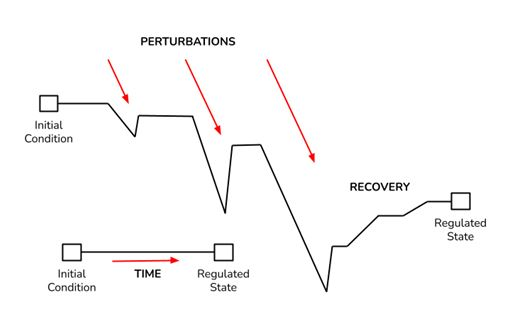
\includegraphics[width=0.7\columnwidth]{figures/fig1}
  \caption{A non-technical example of an AMs internal state trajectory, from initial condition to regulated state. Inset: demonstration of the flow of time, from initial condition to regulated state. }~\label{fig:figure1}
\end{figure}
\subsection{Complexity of the Internal State}
According to Bernard’s naive assumptions about the internal milieu \cite{Ashby:1960:DFB},the selective representations of most cognitive models need to to be considered as a complex, dynamical system. Yet internal states are much more complicated than the output of a simple dynamical system. Based on the variety of internal models featured in the neuroscience literature, such as those representing the cerebellum \cite{wolpert} and attention schema for subjective processing \cite{graziano}, internal models generate representations of cognitive states that are directly relevant to behavioral outputs. As such, they could be defined as invariant to physiological states or innate mechanisms that might influence this state. This becomes important when we take into consideration regulatory mechanisms that determine an individual’s internal state as it actively explores its environment. \\
These innate mechanisms can be represented in a number of ways. Computational representations of the genome \cite{albert}, \cite{aguilar}, particularly gene expression networks (GRNs, see \cite{cussat}), can approximate both the constraints and adaptive capacity of an organism’s internal biology on processing environmental inputs. Particularly interesting in the phenomenon of synthetic effects that occur when multiple genes interact with each other \cite{sanford}. This level of description is utilized in AMs to facilitate robust and vulnerable responses to environmental perturbations. Nonlinear effects also emerge from this level of biopsychological description as gene expression interacts richly with the multiple sensory channels of naturalistic interaction with the environment.


\subsection{Event-oriented trajectory of Internal State}

The main difference between an event-oriented trajectory and a goal-directed one is that event-oriented trajectories are open-ended \cite{adam} dynamical summaries of the internal state. it is possible to revise the Figure 1 in the following way: we might request a more concrete definition of an environmental perturbation. One possible definition, rooted in Psychophysics, is a sensory signal that changes its magnitude with respect to time. Moving your fingertips over a ridged surface results in environmental perturbations of a given frequency and duration because perturbation frequency depends upon the spatial location of each ridge as well as the temporal interval between each ridge. This is further dependent on the speed of the touch effector, which is modulated by feedback from the nervous system. By contrast, perturbation duration involves both speed of the touch effector and the overall capacity of the internal state to withstand perturbations. In essence, this can be reduced to a simple oppositional relationship: robustness of the internal state and its trajectory versus the magnitude/duration of perturbation. \\
From this definition we can understand several components that influence the dynamical trajectory of our AM. Figure 2 demonstrates these steps in graphical form. The first step is to establish a baseline state (Figure 2a). Then a single perturbation of a given strength is delivered to the internal state (Figure 2b). This magnitude has an effect on the strength of a single perturbation (Figure 2c), which drives the state away from the baseline in a negative direction. Perturbation depth is generally at a 45 degree angle to the baseline function, but can be characterized by variable phase angles depending on whether the perturbation is encountered in a gradual or sudden manner. In our haptic ridges example, perturbations are rather sharp. By contrast, haptic exploration of a thermal gradient would be more gradual. \\
\begin{figure}[h]
\centering
  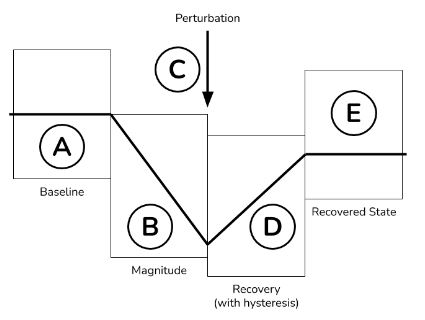
\includegraphics[width=0.7\columnwidth]{figures/fig2}
  \caption{A diagram of the external perturbation/internal state trajectory relationship. Lack of recovery capacity (e.g. hysteresis) of our internal state trajectory is equivalent to allostatic drive}~\label{fig:figure2}
\end{figure}

This leads us to a refractory period, during which the state trajectory generally recovers at a symmetrical phase angle to the perturbation (Figure 2d). Once again, this can depend on the application context. However, the recovery of an internal state trajectory does not always result in a return to the baseline state. When recovery is not equivalent to perturbation strength, then the trajectory is said to be hysteretic. Hysteresis might result from multiple perturbations in rapid succession, or from an insufficient memory of the previous state. The latter will be common for out-of-distribution magnitudes. Finally, the recovered internal state trajectory (Figure 2e) is dependent upon the timing of additional perturbations, which can determine the likelihood of transition to a new state. In material science, hysteresis is often referred to as a form of memory \cite{ortin}. While a memory system is not made explicit in AMs, they nevertheless serve an integral role of their function.\\
One area for further understanding is how to characterize the relative strength of a perturbation. Even when perturbations are described in terms of single sensations (quantities such as Newtons or Lumens), it is hard to describe their effect on the internal state. One way to do this is to define the baseline state as a mean background level of some sensory channel, with local deviations from this value as a perturbation of magnitude \textit{m}. Corresponding to this is a distribution function that can be estimated for the organism or agent that describes a general degree of robustness to outliers, rare events, and out-of-distribution phenomena.


\subsection{Examples from Specific Environmental Representations}
AMs are broadly applicable to a wide range of Neuro-HCI systems. Our approach is particularly amenable to naturalistic experiments, where organisms or agents are allowed to freely explore their environment. Future work will also include the study of cognitive phenomena such as visual flow and spatial cognition. In these cases, perturbations would be introduced through controlled misalignments of visual cues and affordances. This will require the integration of AMs with agent-based models such as developmental Braitenberg Vehicles \cite{bradly_categories} or serve as predictive models for Neuroimaging and Psychophysiological data. \\
Our AM models are also greatly relevant to the study of virtual environments. With respect to hyperrealistic virtual environments, perturbations might take the form of latencies and stimuli of differential resolution. More impressionistic and fantastical virtual representations are less dependent on being as faithful to realism. However, affordances are still required to navigate the environment, and disruptions to their recognizability and relative location may serve to introduce perturbations of different frequencies and magnitudes. 

\section{Discussion}




% Use a numbered list of references at the end of the article, ordered
% alphabetically by first author, and referenced by numbers in
% brackets~\cite{ethics, Klemmer:2002:WSC:503376.503378,
%   Mather:2000:MUT, Zellweger:2001:FAO:504216.504224}. For papers from
% conference proceedings, include the title of the paper and an
% abbreviated name of the conference (e.g., for Interact 2003
% proceedings, use \textit{Proc. Interact 2003}). Do not include the
% location of the conference or the exact date; do include the page
% numbers if available. See the examples of citations at the end of this
% document. Within this template file, use the \texttt{References} style
% for the text of your citation.

% Your references should be published materials accessible to the
% public.  Internal technical reports may be cited only if they are
% easily accessible (i.e., you provide the address for obtaining the
% report within your citation) and may be obtained by any reader for a
% nominal fee.  Proprietary information may not be cited. Private
% communications should be acknowledged in the main text, not referenced
% (e.g., ``[Robertson, personal communication]'').

AMs are decoupled from measurements of neuronal or network output state, which makes them controversial as a model of intelligent behavior. However, such models are differentiable and allow us to understand the mapping between internal state and the effects of a naturalistic environment. We can also use AMs to understand the effects of feedback at multiple temporal scales. This might be useful in the approximation of phenomena such as predictive processing \cite{nave}. Indeed, AMs allow for both minimal representational capacity and evaluation of error minimization \cite{williams}. It is important to stress that “evaluation” does not imply optimization: in the case of virtual environments, selective mismatch might be a desirable feature of the interaction. 
\\
Furthermore, considering AMs from the perspective of existing theoretical work on embodied interaction is also important. While we define a simple duality between an internal model and the external environment, affordances encountered in the environment present three- way interactions between an internal model, an external environment, and the body (morphology) itself \cite{Dourish:2001:WAI}. While morphology mediates the interaction between internal and external worlds in this relationship, representations of internal state serve to mediate between innate mechanisms and environmental stresses. AMs might also help us understand how technology usage interplays with the internal state. The idea that technology becomes incorporated into the body over time \cite{clark} can be demonstrated quantitatively using the AM approach.\\
Moreover, AMs can also be applied to a broad range of agent-based settings, from social interaction to tests of biopsychological variation across a common set of interactions. In the case of social interaction, the AMs of different individuals can be compared during cooperation and competition. AMs also lend themselves to understanding the psychophysiology of cognitive states, particularly during continuous tasks like driving \cite{lohani}. We can even use AMs as the basis for game-theoretic analysis, as switching between various internal states can be modeled as a strategic pursuit. In conclusion, it is possible to use agent-based modeling approaches to better understand variation in AMs with respect to the potential difficulty of an environment given a large number of possible internal representations.   

\section{Acknowledgments}

Sample text: We thank attendees of the Saturday Morning NeuroSim group and members of the Orthogonal Research and Education Laboratory Slack for their input.

% Balancing columns in a ref list is a bit of a pain because you
% either use a hack like flushend or balance, or manually insert
% a column break.  http://www.tex.ac.uk/cgi-bin/texfaq2html?label=balance
% multicols doesn't work because we're already in two-column mode,
% and flushend isn't awesome, so I choose balance.  See this
% for more info: http://cs.brown.edu/system/software/latex/doc/balance.pdf
%
% Note that in a perfect world balance wants to be in the first
% column of the last page.
%
% If balance doesn't work for you, you can remove that and
% hard-code a column break into the bbl file right before you
% submit:
%
% http://stackoverflow.com/questions/2149854/how-to-manually-equalize-columns-
% in-an-ieee-paper-if-using-bibtex
%
% Or, just remove \balance and give up on balancing the last page.
%
\balance{}


% BALANCE COLUMNS
\balance{}

% REFERENCES FORMAT
% References must be the same font size as other body text.
\bibliographystyle{SIGCHI-Reference-Format}
\bibliography{sample}

\end{document}

%%% Local Variables:
%%% mode: latex
%%% TeX-master: t
%%% End:
